\documentclass{standalone}

\usepackage{tikz}
\usetikzlibrary{arrows.meta}

\begin{document}

	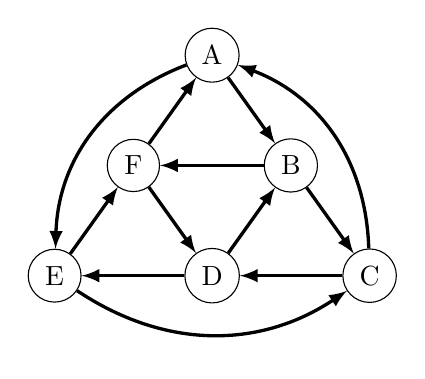
\begin{tikzpicture}
		\node[draw, circle]  (A) at (0,0) {A};
		\node[draw, circle]  (B) at (1,-1.4) {B};
		\node[draw, circle]  (C) at (2,-2.8) {C};
		\node[draw, circle]  (D) at (0,-2.8) {D};
		\node[draw, circle]  (E) at (-2,-2.8) {E};
		\node[draw, circle]  (F) at (-1,-1.4) {F};
		\draw[very thick,  -latex] (A) to (B);
		\draw[very thick,  -latex] (B) to (C);
		\draw[very thick,  -latex] (C) to (D);
		\draw[very thick,  -latex] (D) to (E);
		\draw[very thick,  -latex] (E) to (F);
		\draw[very thick,  -latex] (F) to (A);

		\draw[very thick,  -latex] (A) to [bend right=33.75] (E);
		\draw[very thick,  -latex] (B) to (F);
		\draw[very thick,  -latex] (C) to [bend right=33.75]  (A);
		\draw[very thick,  -latex] (D) to (B);
		\draw[very thick,  -latex] (E) to [bend right=33.75]  (C);
		\draw[very thick,  -latex] (F) to (D);

	\end{tikzpicture}

\end{document}